\chapter{Calibrated Drift Detection Method} \label{chapt:CDDM}

In this chapter we introduce calibrated drift detection method (CDDM), a drift detection method which detects increases in the irreducible error rate, rather than the overall error rate. Section \ref{CDDM:motivation} motivates the approach to concept drift detection taken by CDDM. Section \ref{cddm:setting} discusses the setting and notation of CDDM. Section \ref{CDDM:algorithm} provides the actual CDDM algorithm. Section \ref{CDDM:limitations} discusses theoretical and practical limitations of CDDM. Section \ref{CDDM:conclusion} summarises this chapter and discusses future work. 

%-------------------------------------------------------------------
% MOTIVATION
%-------------------------------------------------------------------

\section{Motivation} \label{CDDM:motivation}

Most, if not all, extant drift detectors assume that significant increases in the error rate of the base learner are due to concept drift and require model retraining. For example, Gama et al. \cite{DDM} state 
\begin{displayquote}
    Statistical [sic] theory \cite{statistical_theory} guarantees that while the class distribution of the examples is stationary, the error rate of the learning algorithm ($p_i$) will decrease when $i$ increases. A significant increase in the error of the algorithm, suggest a change in the class distribution, and that the actual decision model is not appropriate.
\end{displayquote}

\noindent However, this assumption is invalid in environments when 1) some labels can be predicted more easily than others, and 2) feature drift occurs. Consider the following (fictional) example from our motivating domain of medical triage:
\begin{displayquote}
    At a coronavirus emergency clinic, patients with coronavirus symptoms are being triaged. Young patients have a low mortality rate from coronavirus so are given low priority. Old patients have a high mortality rate so are given high priority. Middle aged patients, however, may have high or low mortality depending on other factors, so may be given a high, low, or medium priority. 
    
    The learner is easily able to discover the relationship between age and priority, but fails to make use of other features. The model thus has a higher error rate for middle aged patients than young or old patients. If there is an increase in the number of middle aged patients with coronavirus, then the overall error rate of the model will increase.  
    
    A concept drift detector will detect the increase in the error rate and signal that the model requires retraining. However, because the actual relationship between instances and labels has not changed, retraining the model would at best be a waste of time, and at worst result in an inferior model trained on a smaller dataset. 
    
    Conversely, suppose that instead of an increase in the middle aged patients there is a {\it decrease in middle aged patients}. This will reduce the average difficulty of the prediction task, and reduce the error rate of the model. 
    
    Suppose that shortly after this occurs, the clinic decides to change its triage policy for dealing with middle aged patients. Because the model is trained to implement the old policy, its error rate for middle aged patients will further increase, but this increase may be cancelled out by the decrease from the reduced number of middle aged patients. 
    
    Thus, a concept drift detector may fail to notice the real drift which has occurred, and the model will not be retrained despite the change in the decision boundary. This situation may therefore result in a false negative.
\end{displayquote}
This example illustrates that a concept drift detector should not monitor for increases in the error rate of the model {\it per se}. Instead it should monitor for increases in rate of {\it reducible} error due to {\it real} drift which is {\it not} predictable {\it ex ante} from the prediction task becoming more difficult on average. An increase in the {\it irreducible} error due to {\it virtual} drift which {\it is} predictable {\it ex ante} is a confounder. It can cause false negatives and false positives, such that the model may not be retrained when it should be, and may be retrained when it does not need to be.

%-------------------------------------------------------------------
% SETTING
%-------------------------------------------------------------------

\section{Setting} \label{cddm:setting}

Let $y$ be the true label given to some instance $x$, and $\hat{y}$ be the label predicted by the model. Due to noise, stochasticity, or the limited inferential capabilities of the learner, there is some probability that the model will make the wrong prediction. We thus denote
\begin{equation}
q = \Pr(y=\hat{y})
\end{equation}
as the {\bf reliability} of the model, or the probability that the model will make the correct prediction, for the given instance. 

We assume our model makes probabilistic predictions. We can thus talk about the model {\bf confidence} as the probability assigned by the model to its predicted label, denoted
\begin{equation}
\hat{q} = \hat{\Pr}(y=\hat{y}).
\end{equation}
A plot of a model's confidence versus its reliability is called a {\bf reliability diagram} \cite{calibrating}, and is illustrated in Figure \ref{fig:calibration}. 

\newcommand{\calibrationgraph}[7][]{
    % args:
    \draw [thick, <->] (0,1.25) -- (0,0) -- (1.25,0);
    \node [below] at (1.25,0) {$\hat{q}$};
    14
    \node [left] at (0,1.25) {$q$};
    \node [left] at (0,#7) {$q_t$};
    \node [below] at (#6,0) {$\hat{q}_t$};
    \draw (#2,#3) -- (#4,#5);
    \draw [red] (#6,0) -- (#6,#7);
    \draw [red, dashed] (0,#7) -- (#6,#7);
}

\begin{figure}
    \centering
    \begin{tikzpicture}[scale=3]
        \calibrationgraph{0}{0}{1}{1}{0.5}{0.5}
    \end{tikzpicture}
    \caption{Calibration Graph}
    \label{fig:calibration}
\end{figure}

When a model's confidence is equal to its reliability, $q=\hat{q}$, we say that the model is {\bf calibrated} \cite{superforecasting}\cite{scoring_rules}\cite{calibrating}. For example, if a calibrated model makes 10 predictions, and assigns a 0.9 confidence to each of them, then in expectation, one of those predictions will turn out to be incorrect. The reliability diagram in Figure \ref{fig:calibration} is of a calibrated model, as it shows an identity relationship between confidence and reliability.

\newcommand{\calibrationgraphB}[7][]{
    % args:
    \draw [thick, <->] (0,1.25) -- (0,0) -- (1.25,0);
    \node [below] at (1.25,0) {$\hat{q}$};
    14
    \node [left] at (0,1.25) {$q$};
    \node [left] at (0,#7) {$Acc$};
    \node [below] at (#6,0) {$\mathbb{E}[\hat{q}]$};
    \draw (#2,#3) -- (#4,#5);
    \draw [red] (#6,0) -- (#6,#7);
    \draw [red, dashed] (0,#7) -- (#6,#7);
}

\newcommand{\virtualdriftgraph}[3][]{
    \begin{tikzpicture}[scale=3]
        \calibrationgraphB{0}{0}{1}{1}{0.5+#2}{0.5+#2}
        \draw [red, thick, ->] (0.5, #3) -- (0.5+#2*1.5, #3);
    \end{tikzpicture}
}

\begin{figure}
    \centering
    \begin{tikzpicture}[scale=3]
        \calibrationgraphB{0}{0}{1}{1}{0.5}{0.5}
    \end{tikzpicture}
        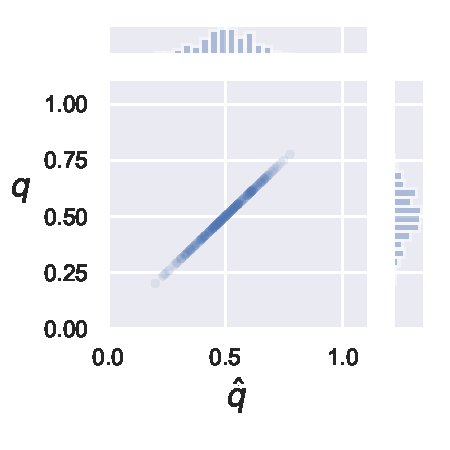
\includegraphics[width=0.3\textwidth]{images/no_drift.pdf}
    \caption{A calibrated model.}
    \label{fig:no_drift}
\end{figure}

When a model is calibrated, we can estimate the accuracy and error rate of the model from its confidence. Figure \ref{fig:no_drift} shows a reliability diagram plus the distribution over confidence values, and thus the distribution over reliability. The accuracy is the expected value of the reliability 
\begin{equation}
    Acc = \mathbb{E}[q]
\end{equation}
and the error rate is one minus the accuracy:
\begin{equation}
    Err = 1 - Acc = \mathbb{E}[q].
\end{equation}
In this manner we may derive an {\it ex ante} estimation of the model's accuracy based on its confidence scores. If the actual {\it ex post} accuracy significantly deviates from this accuracy, then we have evidence that the model is miscalibrated, which we take as evidence of concept drift.

Suppose the average difficulty of the prediction task increases, as described in Section \ref{CDDM:motivation}, and illustrated in Figure \ref{fig:pos_virt}. A calibrated model will decrease in its mean confidence, and our {\it ex  ante} expected error rate will increase. When we observe an {\it ex post} increase in the error rate we will know that this can be attributed to feature drift rather than due to real drift, and so the model should not be retrained. In other words, we have observed an increase in the irreducible error rather than reducible error. We can thus avoid false positive.

\begin{figure}
    \centering
    \virtualdriftgraph{-0.2}{0.125}     
    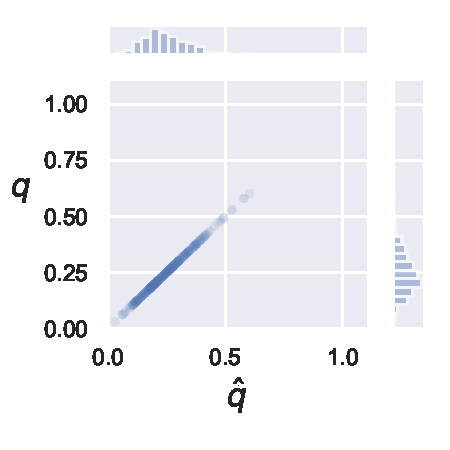
\includegraphics[width=0.3\textwidth]{images/positive_virtual.pdf}
    \label{fig:pos_virt}
    \caption{An increase in irreducible error rate.}
\end{figure}

Conversely, consider the other case described in Section \ref{CDDM:motivation} and illustrated in Figure \ref{fig:co_drift}, where the average difficulty of the prediction task decreases around the same time as real drift occurs. In this case the mean confidence of the model decreases, and so {\it ex ante} error rate decreases. If the {\it ex post} error rate does not decrease, this indicates that concept drift has occurred. In other words, there has been an increase in the reducible error rate, but it has been obscured by a decrease in the irreducible error rate. We can thus detect that the model {\it should} be retrained despite no increase in the overall error rate and thus avoid a false negative.

\begin{figure}
    \centering
    \begin{tikzpicture}[scale=3]
        \calibrationgraphB{0.25}{0}{1}{0.75}{0.75}{0.5}
        \draw [black, thick, ->] (0.9, 0.8) -- (0.9, 0.5);
        \draw [red, thick, ->] (0.6, 0.2) -- (0.85, 0.2);
    \end{tikzpicture}
        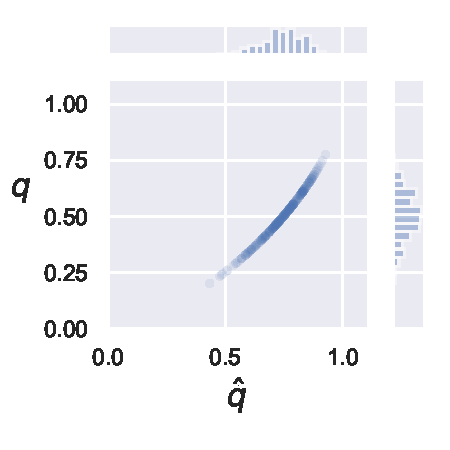
\includegraphics[width=0.3\textwidth]{images/hidden_drift.pdf}
    \caption{A decrease in irreducible error masking an increase in reducible error.}
    \label{fig:co_drift}
\end{figure}

%-------------------------------------------------------------------
% ALGORITHM
%-------------------------------------------------------------------

\section{Algorithm} \label{CDDM:algorithm}

CDDM detects increases in reducible error rather than overall error by monitoring for differences in the {\it ex ante} accuracy and the {\it ex post} accuracy. 

Intuitively, we can consider CDDM to be placing a ``bet" on each prediction. If the model has confidence $\hat{q}$ in its prediction, then it will buy a bet that it is correct for \$$\hat{q}$. If the prediction turns out to be correct, the model will receive a payoff of \$1, otherwise it will receive a payoff of \$0. The payoff is denoted:
\begin{equation}
    \gamma = \begin{cases} 
        1-\hat{q} & \text{if }y=\hat{y} \\ 
        -\hat{q} & \text{if }y\ne\hat{y}
    \end{cases}
\end{equation}
The expected value of the payoff under normal, calibrated conditions is zero:
\begin{align}
	\mathbb{E}[\gamma] &= \Pr(y=\hat{y}) \cdot (1-\hat{q}) - \Pr(y\ne \hat{y}) \cdot \hat{q} \\
	&= q \cdot (1-q) - (1-q) \cdot q \\
	&= 0. \label{eq:expectation}
\end{align}
If we have observed $n$ payoffs, $\gamma_1,\gamma_2,\dots,\gamma_n$, then we can use Hoeffding's inequality \cite{hoeffding} to bound the probability of seeing a large average payoff:
\begin{align}
    \Pr\left(  \left| \frac{1}{n} \sum_{i=1}^n \gamma_i - \mathbb{E}\left[\frac{1}{n} \sum_{i=1}^n \gamma_i\right] \right| \ge k \right)
    &= \Pr\left(  \left| \frac{1}{n} \sum_{i=1}^n \gamma_i \right| \ge k \right) \\
    &\le 2 \exp\left(-\frac{2n^2k^2}{\sum_{i=1}^n(b_i - a_i)^2}\right) \\
    \intertext{Where $a_i$ and $b_i$ are lower and upper bounds on $\gamma_i$, respectively. Because $0\le \hat{q} \le 1$, we have $a_t=-1 \le \id{y_t=\hat{y}_t} - \hat{q}_t \le b_t=1$.}
  &\le \exp\left(-\frac{2n^2k^2}{\sum_{i=1}^n 4}\right) \\
  &\le \exp\left(-\frac{nk^2}{2}\right). \label{eq:hoeffding}
\end{align}
CDDM maintains a sliding window of the most recent $n$ payoff values. Equation \ref{eq:hoeffding} gives a $p$-value for an average payoff across this window at least as extreme as observed. If this value falls below some critical threshold, we may reject the null hypothesis and conclude that the model is miscalibrated. In this case, CDDM will signal that drift has occurred.

Similar to several other drift detectors \cite{DDM}\cite{HDDM}\cite{FLORA}, we use two critical thresholds: $\alpha_{warn}$, a warning threshold, and $\alpha_{drift}$, a drift threshold. When the $p$-value falls below $\alpha_{warn}$, CDDM emits a warning that drift may be occurring, and all new instances are placed in a buffer. When the $p$-value falls below $\alpha_{drift}$, CDDM indicates that concept drift has occurred. The model is then retrained on the instances in the buffer. The full pseudocode is given in Algorithm \ref{alg:cddm_basic}.

\begin{algorithm}
    \caption{CDDM algorithm}
    \label{alg:cddm_basic}
    \begin{algorithmic}
    \Require Warning threshold $\alpha_{warn}$
    \Require Drift threshold $\alpha_{drift}$
    \Require Window size $N$
    \State Window $\gets$ []
    \State {\tt status} $\gets$ {\tt normal}
	\For {$y_t, \hat{q}_t, \hat{y}_t$ in the data stream}
        \State $\gamma_t \gets \id{y=\hat{y}} - \hat{q}$
        \State Window $\gets \{\gamma_t\} \cup$ Window
        \State $n =$ Window.length
        \If {$n > N$}
            \State Window.pop()
        \EndIf
        \State $k \gets \left| \text{Window.mean} \right|$
        \State $p \gets 2\exp\left(-\frac{nk^2}{2}\right)$
        \If {$p \leq \alpha_{drift}$}
            \State {\tt status} $\gets$ {\tt drift}
        \ElsIf {$p_{min} \leq \alpha_{warn}$}
            \State {\tt status} $\gets$ {\tt warn}
        \EndIf
    \EndFor
    \end{algorithmic}
\end{algorithm}

%-------------------------------------------------------------------
% LIMITATIONS
%-------------------------------------------------------------------

\section{Limitations} \label{CDDM:limitations}

CDDM suffers from two major limitations. The first is that CDDM requires learners to be calibrated, but most machine learning algorithms are not calibrated out of the box. The second is that small deviations from calibration will not be detectable by CDDM.

\subsection{Calibration}

CDDM requires the base learner to be calibrated. In fact few machine learning models are calibrated out of the box, and require post-hoc transformations of  their probabilistic predictions to become calibrated.

Some models are ``overconfident", meaning that the model's confidence tends to exceed its reliability, $\hat{q}>q$. Some deep learning models such as LeNet \cite{lenet} suffer from overconfidence \cite{nn_calibration}.

Conversely, some models are ``underconfident", meaning that the model's reliability tends to exceed its confidence, $\hat{q}<q$. Some deep learning models such as ResNet \cite{resnet} suffer from underconfidence \cite{nn_calibration}.  

Other models tend to ``extremism", meaning that they are underconfident for confidences close to 0, and overconfident for confidences close to 1.  Extremist models can be considered as pushing $\hat{q}$ values towards 0 and 1 with respect to $q$ values. Maximum margin methods such as boosted trees and boosted stumps are prone to extremism \cite{calibrating}.

The opposite behaviour to extremism is ``moderatism", meaning the model is underconfident for confidence values close to 1 and overconfident for confidence values close to 0. Thus, $\hat{q}$ values are pushed {\it away from} 0 and 1 with respect to $q$ values. Na\"{i}ve Bayes models are prone to moderatism due to making unrealistic independence assumptions \cite{calibrating}. 

The terms ``overconfident" and ``underconfident" are standard in the prediction literature \cite{superforecasting}. ``Extremism" and ``moderatism" are our own terminology. These behaviours are illustrated with reliability diagrams in Figure \ref{fig:calib_drift_types}. 

\begin{figure}%[t!]
    \centering
    \subfigure[Underconfidence]{
        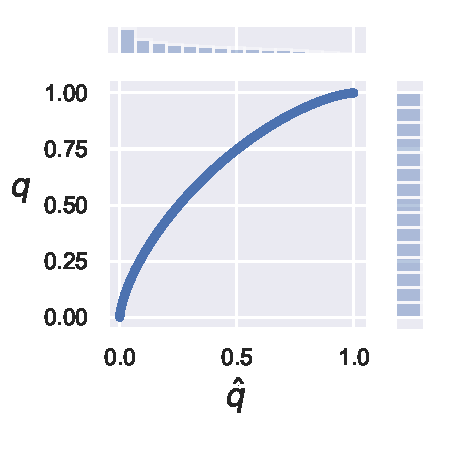
\includegraphics[width=0.45\textwidth]{images/overconfident.pdf}
    }
    \subfigure[Overconfidence]{
        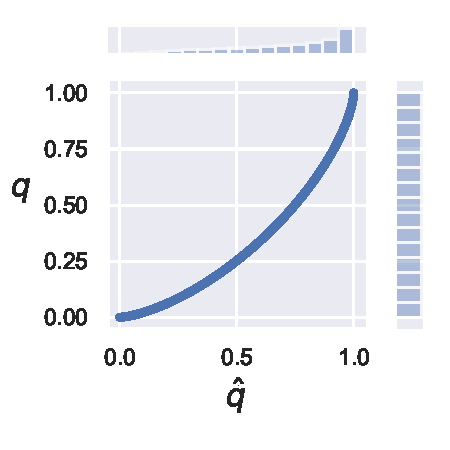
\includegraphics[width=0.45\textwidth]{images/underconfident.pdf}
    }
    \subfigure[Extremism]{
        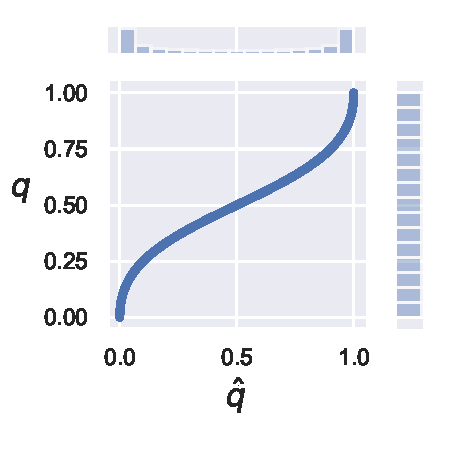
\includegraphics[width=0.45\textwidth]{images/extremist.pdf}
    }
    \subfigure[Moderatism]{
        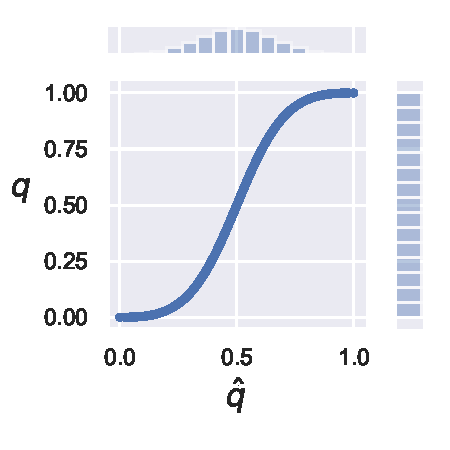
\includegraphics[width=0.45\textwidth]{images/moderate.pdf}
    }
    \caption{Reliability diagrams for a common model behaviours.}
    \label{fig:calib_drift_types}
\end{figure}

Models are often not calibrated because they are designed to optimise some metric other than calibration, such as accuracy. However, even in cases where models {\it are} optimised for calibration, miscalibration can still occur. For example, minimising cross entropy is a standard optimisation objective in deep learning \cite{deep_learning}. This is a proper scoring rule \cite{scoring_rules}, so this optimisation encourages both calibration and accuracy. However, many deep learning models still fail to calibrate \cite{nn_calibration}. This may be due to lack of robustness against dataset shift \cite{dataset_drift}, or overfitting the training data \cite{nn_calibration}.

A model which is not calibrated can be remedied by applying a post-processing function to a model's probabilistic predictions. This function is called a {\bf calibration map} \cite{calibrating}. A variety of methods for generating calibration maps have been developed. Some of the major methods are given below.

Logistic calibration - also called {\bf Platt scaling} \cite{platt} fits a sigmoid function, given by
\begin{equation}
	q = \frac{1}{1 + \exp(a\hat{q} + b)}
\end{equation}
to model probabilities. The parameters $a$ and $b$ are fitted using maximum likelihood estimation on a calibration set. Logistic calibration tends towards exactly correct calibration when the model's confidence values are normally distributed \cite{beyond_sigmoids}. 

Isotonic calibration is a non-parametric type of calibration map \cite{isotonic_calibration}. It is therefore more flexible than logistic calibration, but more prone to overfitting. The only assumption isotonic regression makes about the reliability diagram is that it is isotonic, that is, it is monotonically increasing. 

Beta calibration is a generalisation of sigmoid calibration \cite{beyond_sigmoids}. A beta calibration map takes the form
\begin{equation}
	q = \frac{1}{1 + 1/\left(e^c\frac{\hat{q}^a}{(1-\hat{p})^b}\right) }
\end{equation}
where $a,b\ge 0$ so that the map is monotonically non-decreasing. This map can be fitted as easily as a logistic map \cite{beyond_sigmoids}. Beta calibration is intended to overcome some of the drawbacks of logistic calibration, such as distortions for many classifiers including Naive Bayes and Adaboost. Beta calibration tends towards exactly correct calibration when the model's confidence values are beta distributed. Experiments have found beta calibration to be superior to logistic calibration for Na\"{i}ve Bayes, Adaboost, Random Forests, logistic regression, support vector machines, and multilayer perceptrons \cite{beyond_sigmoids}. 

Other calibration map methods include histogram binning \cite{histogram_calibration}, Bayesian binning into quantile (BBQ) \cite{bbq_binning}, matrix and vector scaling \cite{nn_calibration}, and temperature scaling \cite{nn_calibration}\cite{temperature_scaling}.

\subsection{Small Deviations from Calibration}

CDDM cannot detect small deviations from calibration. Suppose the base learner has been calibrated up to time $t-n$, and from $t-n$ to $t$ it has been slightly overconfident (or underconfident). Specifically,
\begin{equation}
    \delta_i = \begin{cases}
        0 & 0 \le i < t-n \\ 
        \left| \hat{q}_i - q_i \right| & t-n \le i < t
    \end{cases}
\end{equation}
Given a window size $N$, the miscalibration will be on the cusp of detectability from CDDM when the $p$-value given by equation Equation \ref{eq:hoeffding} is equal to the drift detection threshold $\epsilon$: 
\begin{equation}
    \epsilon = \exp\left(-\frac{n^2\delta^2}{2N}\right).
\end{equation}
Solving for $\delta$ gives the minimum overconfidence value which can be detected within $n$ time steps for a given drift threshold and window size:
\begin{align}
    \delta &= \sqrt{-\frac{2N}{n^2}\ln\left(\frac{\epsilon}{N}\right)}.
\end{align}
This relationship is plotted for a range of window sizes with drift threshold 0.01 in Figure \ref{fig:cddm_window_size}. In this plot we can see that, for example, an overconfidence of $\delta=0.4$ can be detected within 250 time steps for a window size of 2000.

\begin{figure}
    \centering
    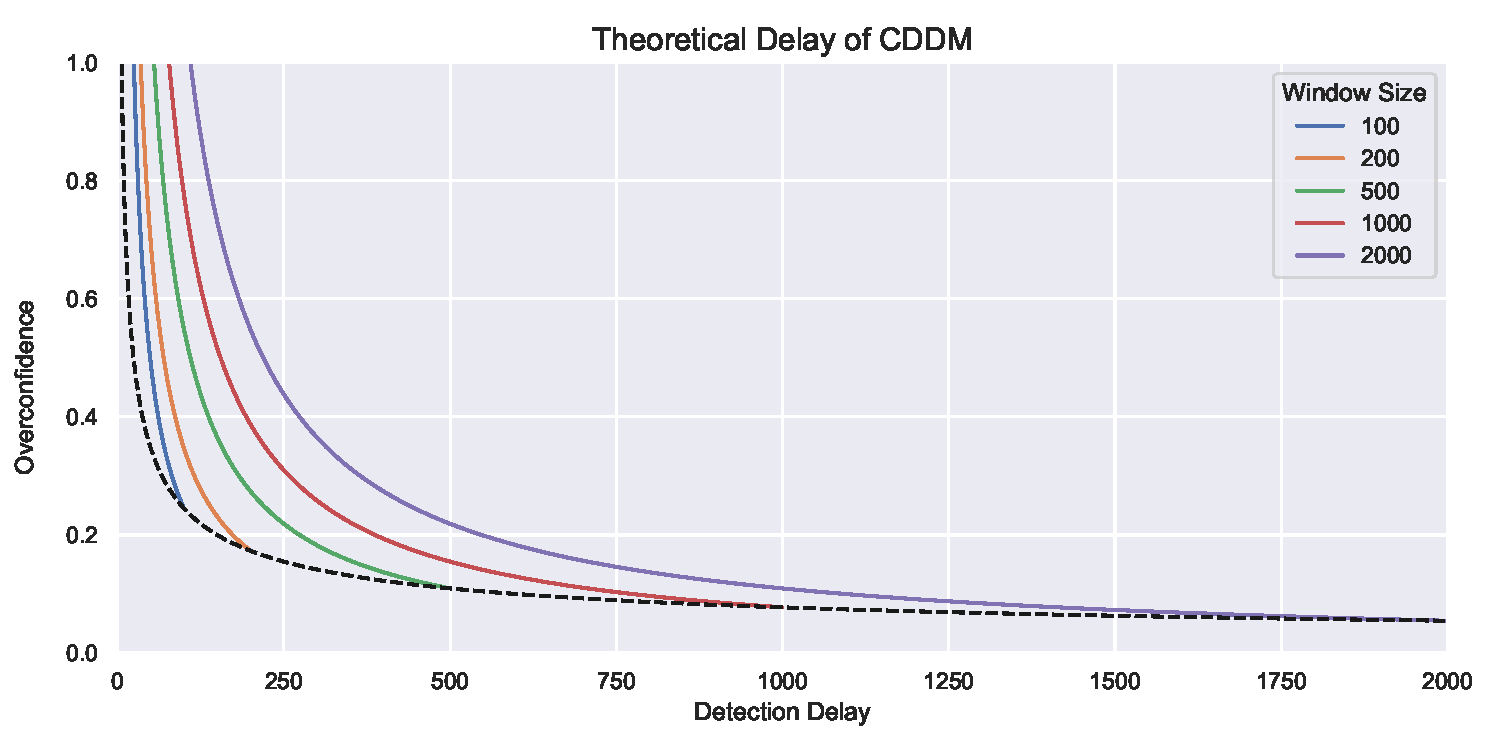
\includegraphics[width=\textwidth]{images/cddm_window_size.pdf}
    \caption{Detection delay versus overconfidence magnitude for CDDM.}
    \label{fig:cddm_window_size}
\end{figure}

The smallest overconfidence value which can possibly be detected by CDDM is found by setting $n=N$. That is, it is only detectable when the entire window has filled up with the miscalibrated payoffs. The range of detectable miscalibrations is thus given by 
\begin{equation}
    1 \ge \delta \ge \sqrt{-\frac{2}{N}\ln\left(\frac{\epsilon}{N}\right)}. \label{eq:window_size}
\end{equation}
The dashed line in Figure \ref{fig:cddm_window_size} indicates this lower bound on detectable miscalibration. This shows that, for example, a miscalibration of magnitude $\delta=0.1$ will be undetectable with a window size of $N=200$.

%-------------------------------------------------------------------
% CONCLUSION
%-------------------------------------------------------------------

\section{Conclusion} \label{CDDM:conclusion}

In this chapter we introduced calibrated drift detection method (CDDM). We argued that a drift detector should detect increases in the reducible error rate rather than the overall error rate, so as to avoid unnecessary retraining. CDDM takes this approach to concept drift detection by detecting when a model becomes miscalibrated. However, CDDM still has some significant limitations. Theoretically, CDDM can only detect mean overconfidence below a certain level determined by the window length. Practically, CDDM assumes that a learner is initially calibrated, whereas most models require prediction post-processing to achieve calibration.

A promising direction for future work would be building a calibration map online, and detecting when this calibration map changes, rather than assuming the learner is calibrated in the first place.